\setcounter{page}{1}

\renewcommand{\thefigure}{S\arabic{figure}}
\setcounter{figure}{0}
\renewcommand{\thesection}{S\arabic{section}}
\setcounter{section}{0}
\renewcommand{\thetable}{S\arabic{table}}
\setcounter{table}{0}

\begin{center}
\Large\textbf{Bridging LLM Emotion Representations and EEG}\par
\vspace{0.5em}
\Large Supplementary Material
\end{center}

\noindent In this supplementary document, we include:
\begin{itemize}
    \item \textbf{Section \ref{sec:supp_exp}:} Full experimental details and hyperparameters.
    \item \textbf{Section \ref{sec:supp_arch}:} Complete architecture experiment results.
    \item \textbf{Section \ref{sec:supp_llm}:} Multi-LLM emotion vector analysis (11 instruction-tuned models).
    \item \textbf{Section \ref{sec:supp_midlayer}:} Mid-layer extraction sweep across Qwen and Gemma-4.
    \item \textbf{Section \ref{sec:supp_seedv5s}:} SEED-V 5\,s preprocessing details and full per-seed results.
    \item \textbf{Section \ref{sec:supp_efficiency}:} Computational efficiency breakdown.
    \item \textbf{Section \ref{sec:supp_labram_recipes}:} LaBraM KD recipe robustness across three variants.
    \item \textbf{Section \ref{sec:supp_per_subject}:} Per-subject KD benefit distribution.
    \item \textbf{Section \ref{sec:supp_eegdino}:} EEG-DINO third cross-backbone and token-count confirmation.
    \item \textbf{Section \ref{sec:supp_reve}:} REVE replication attempt.
    \item \textbf{Section \ref{sec:supp_baseteachers}:} Non-instruction-tuned teacher controls.
    \item \textbf{Section \ref{sec:supp_sft}:} Emotion-specific SFT of the teacher.
    \item \textbf{Section \ref{sec:supp_seedv_loso}:} SEED-V cross-subject leave-group-out.
    \item \textbf{Section \ref{sec:supp_peft_dataset}:} Dataset-dependent PEFT.
    \item \textbf{Section \ref{sec:supp_best_teacher}:} Best-teacher comparison.
    \item \textbf{Section \ref{sec:supp_llama4}:} Llama-4 Scout loading issue.
    \item \textbf{Section \ref{sec:supp_explore}:} Additional architecture exploration.
    \item \textbf{Section \ref{sec:supp_negative}:} Comprehensive negative results catalog (Session 24).
    \item \textbf{Section \ref{sec:supp_editing}:} EEG editing experiments and analysis.
    \item \textbf{Section \ref{sec:supp_seedv_decomp}:} SEED-V gain decomposition.
\end{itemize}

\section{Experimental Details}
\label{sec:supp_exp}

\noindent\textbf{Hardware.} All experiments were run on NVIDIA V100 (32GB) and A100 (80GB) GPUs on the IBEX cluster at KAUST. Training time per CBraMod FACED experiment: $\sim$50 minutes (50 epochs $\times$ 1\,min/epoch). LaBraM and SEED-V experiments: similar wallclock. Total compute for the entire study: $\sim$350 GPU-hours across 70+ configurations and $>$500 individual training runs.

\noindent\textbf{Hyperparameters.} AdamW optimizer with multi-LR (backbone $10^{-4}$, heads $5 \times 10^{-4}$), cosine annealing to $10^{-6}$, weight decay $0.05$, gradient clipping $1.0$, batch size 64, dropout $0.1$, label smoothing $0.1$. We use 50 epochs for all main results; training-duration ablations confirmed convergence by epoch 50 ($+0.1\%$ at 100 epochs is within noise).

\noindent\textbf{Seeds.} All main results use 5 random seeds: 3407, 42, 123, 456, 789. We additionally compute paired bootstrap 95\% percentile CIs (10{,}000 resamples) for all critical comparisons.

\noindent\textbf{Emotion vector extraction.} For each emotion class, we generate 30 short ($\leq$150 tokens) stories using the prompt template ``Write a very short paragraph (3--4 sentences) about \{topic\} where a character experiences intense \{emotion\}. Show the emotion through actions and reactions.'' across 30 diverse topics (e.g., ``a morning commute,'' ``a hospital visit''). Hidden states are extracted from a configurable layer (default: 67th-percentile of total layers), averaged across all token positions excluding the first 50 prompt tokens, and averaged across all 30 stories. We then subtract the global mean across all emotions to obtain contrast vectors and L2-normalize them.

\noindent\textbf{LLM teacher choice.} The main paper uses Qwen2.5-0.5B-Instruct ($D = 896$, layer 21 of 24 = 87\% depth, the 67th-percentile setting). We tested 7 Qwen2.5 sizes and 4 Gemma-4 variants and verified that the choice does not significantly affect downstream EEG accuracy. Specifically, Qwen-1.5B layer 8 (mid-layer, $D = 1536$) yields $0.628 \pm 0.007$ vs $0.625 \pm 0.003$ for the default Qwen-0.5B 67\% setting---a $+0.4\%$ difference with $p = 0.25$ in a paired test.

\section{Complete Architecture Experiments}
\label{sec:supp_arch}

This section provides the full breakdown of every architecture variant we evaluated on FACED. All rows in \cref{tab:supp_arch} use the same training recipe as our best run (aug $p=0.6$, LLM hidden-state KD, 3-layer BN projection, 50 epochs), so the differences isolate the effect of architecture alone. The table consolidates four ablation families: \textbf{(i) PEFT adapters} with bottleneck rank $r \in \{16, 32, 64, 128\}$ that peaks at $r=64$ ($0.628$); \textbf{(ii) LoRA} at rank $\{4, 8, 16\}$ which is flat around $0.619$; \textbf{(iii) FiLM conditioning} with $3$ or $6$ modulation layers, both underperforming adapters; and \textbf{(iv) Depth reduction} of the pretrained backbone from $12$ to $8$ or $6$ layers, which drops performance to $0.603$ and $0.593$ respectively. We also include two cross-attention read-outs (Perceiver-style~\cite{jaegle2021perceiver} with $K=9$ or $K=16$ learnable queries) that collapse to near-chance, indicating the criss-cross backbone's feature grid is not compatible with a learnable query aggregator in this setting. Three findings stand out. First, adapters with a frozen backbone match or beat full fine-tuning ($0.628$ vs.\ $0.627$) despite training only $0.31$\,M extra parameters. Second, LoRA is strictly worse than adapters across the entire rank range tested. Third, depth matters: removing a third of the encoder layers costs $\sim$$3\%$ balanced accuracy, so the full pretrained depth is load-bearing for the criss-cross attention.

\begin{table}[!h]
\caption{All architecture experiments on FACED (5-seed mean). All experiments use the best training recipe (aug $p = 0.6$, KD, 3L-BN projection).}
\small
\centering
\begin{tabular}{llccc}
\toprule
Category & Method & B.Acc & Std & Trainable Params \\
\midrule
Full FT & KD+aug ($p=0.6$) & 0.627 & 0.004 & 134M \\
\midrule
\multirow{4}{*}{Adapters} & Adapter-16 & 0.616 & 0.004 & 129M + 79K \\
 & Adapter-32 & 0.615 & 0.009 & 129M + 156K \\
 & \textbf{Adapter-64} & \textbf{0.628} & 0.006 & 129M + 310K \\
 & Adapter-128 & 0.622 & 0.008 & 129M + 618K \\
\midrule
\multirow{3}{*}{LoRA} & LoRA-4 & 0.620 & 0.008 & 129M + 19K \\
 & LoRA-8 & 0.618 & 0.007 & 129M + 38K \\
 & LoRA-16 & 0.619 & 0.004 & 129M + 77K \\
\midrule
\multirow{2}{*}{FiLM} & FiLM-3 & 0.612 & 0.008 & 135M \\
 & FiLM-6 & 0.615 & 0.003 & 136M \\
\midrule
\multirow{2}{*}{Depth} & 8 layers & 0.603 & 0.004 & 132M \\
 & 6 layers & 0.593 & 0.006 & 132M \\
\midrule
Cross-Attn & K=9 queries & 0.260 & --- & 6.6M \\
 & K=16 queries & 0.276 & --- & 6.8M \\
\bottomrule
\end{tabular}
\label{tab:supp_arch}
\end{table}

\section{Multi-LLM Emotion Vector Analysis}
\label{sec:supp_llm}

We extract emotion vectors from 11 instruction-tuned models in 2 families plus several control base models. \cref{tab:supp_llm} reports the PC1--valence Pearson $r$, cluster separation ratio, and binary cluster purity for each.

\begin{table}[!h]
\caption{Multi-LLM emotion vector quality. Instruction-tuned Qwen and Gemma-4 models show strong valence structure ($p < 0.001$ for all). Base models (Pythia, Bloom) and small non-instruct models (TinyLlama) lack structure.}
\small
\centering
\begin{tabular}{llcccc}
\toprule
Model & Family & Pearson $r$ & Cluster Sep & $p$-value & Structure? \\
\midrule
\multicolumn{6}{l}{\textit{Qwen2.5 family (7 sizes, 67\%-depth):}} \\
Qwen2.5-0.5B & Alibaba & $0.932$ & $1.74$ & $3 \times 10^{-4}$ & \cmark \\
Qwen2.5-1.5B & Alibaba & $0.955$ & $\mathbf{2.04}$ & $6 \times 10^{-5}$ & \cmark \\
Qwen2.5-3B & Alibaba & $\mathbf{0.976}$ & $1.77$ & $7 \times 10^{-6}$ & \cmark \\
Qwen2.5-7B & Alibaba & $0.941$ & $1.87$ & $2 \times 10^{-4}$ & \cmark \\
Qwen2.5-14B & Alibaba & $0.943$ & $1.81$ & $1 \times 10^{-4}$ & \cmark \\
Qwen2.5-32B & Alibaba & $0.926$ & $1.68$ & $3 \times 10^{-4}$ & \cmark \\
Qwen2.5-72B & Alibaba & $0.965$ & $1.63$ & $3 \times 10^{-5}$ & \cmark \\
\midrule
\multicolumn{6}{l}{\textit{Gemma-4 family (4 variants, best layer for each):}} \\
Gemma-4 E2B (29\%) & Google & $0.913$ & --- & $6 \times 10^{-4}$ & \cmark \\
Gemma-4 E4B (29\%) & Google & $0.896$ & --- & $1 \times 10^{-3}$ & \cmark \\
Gemma-4 26B-A4B (67\%) & Google & $0.881$ & --- & $2 \times 10^{-3}$ & \cmark \\
Gemma-4 31B (67\%) & Google & $\mathbf{0.972}$ & --- & $7 \times 10^{-6}$ & \cmark \\
\midrule
\multicolumn{6}{l}{\textit{Control models (no instruction tuning):}} \\
Mistral-7B-Instruct & Mistral AI & $-0.78$ & --- & $0.013$ & \cmark \\
Phi-2 & Microsoft & $-0.53$ & --- & $0.139$ & Marginal \\
TinyLlama & Meta & $+0.27$ & --- & $0.488$ & \xmark \\
Pythia-1.4B & EleutherAI & $+0.30$ & --- & $0.433$ & \xmark \\
Bloom-560M & BigScience & $0.00$ & --- & $1.000$ & \xmark \\
\bottomrule
\end{tabular}
\label{tab:supp_llm}
\end{table}

\noindent\textbf{Cross-family RDM agreement.} \cref{fig:cross_family_rdm} (main paper) shows the full $11 \times 11$ pairwise RSA matrix. Within-Qwen agreement averages $\rho = 0.883 \pm 0.067$ (42 pairs); within-Gemma $\rho = 0.904 \pm 0.055$ (12 pairs); cross-family Qwen$\leftrightarrow$Gemma $\rho = 0.818 \pm 0.081$ (56 pairs). The strongest cross-family pair is Qwen-0.5B$\leftrightarrow$Gemma-4 26B-A4B at $\rho = 0.971$.

\noindent\textbf{Linear probing.} For each LLM we evaluate (i) PC1--valence Pearson $r$, (ii) leave-one-out nearest-neighbor (cosine) accuracy on valence sign, (iii) k-means cluster purity for the 8-class binary positive/negative split (excluding neutral), and (iv) linear separability via projection onto the (positive mean $-$ negative mean) direction. All Qwen and Gemma-4 instruction-tuned models achieve $\geq$$88\%$ binary cluster purity at appropriate depth, with $100\%$ for Qwen-1.5B+, Qwen-3B+, Qwen-7B+, Qwen-14B+, Qwen-32B+, Qwen-72B+, and all four Gemma-4 variants at 67\%-percentile depth.

\section{Mid-Layer Extraction Sweep}
\label{sec:supp_midlayer}

\begin{table}[!h]
\caption{Mid-layer extraction (29\% depth) for Qwen2.5 family with downstream CBraMod FACED KD evaluation (5 seeds). Qwen-1.5B layer 8 is the best teacher, with paired $t$-test $p = 0.047$ vs.\ Qwen-0.5B layer 6.}
\small
\centering
\begin{tabular}{lccccc}
\toprule
Model & Total Layers & Mid Layer & Mean B.Acc & Std \\
\midrule
Qwen-0.5B & 24 & 6 & 0.6137 & 0.0068 \\
\rowcolor{blond}
\textbf{Qwen-1.5B} & 28 & 8 & \textbf{0.6283} & 0.0065 \\
Qwen-3B & 36 & 10 & 0.6223 & 0.0050 \\
Qwen-7B & 28 & 8 & 0.6193 & 0.0043 \\
Qwen-14B & 40 & 13 & 0.6205 & 0.0049 \\
Qwen-32B & 64 & 18 & 0.6172 & 0.0071 \\
\bottomrule
\end{tabular}
\label{tab:supp_midlayer}
\end{table}

\noindent\textbf{Cross-family observation.} Within Gemma-4, the optimal extraction depth scales with model size: small models (E2B with 35 layers, E4B with 42 layers) achieve their highest valence correlation at 29\%-percentile depth, while large models (26B-A4B with 30 layers, 31B with 60 layers) peak at 67\%-percentile depth ($r = 0.972$ for 31B). For Qwen, all 7 sizes consistently peak at 67\%-percentile depth. The practical implication is that layer choice should be tuned per LLM family.

\section{SEED-V 5\,s Preprocessing and Per-Seed Results}
\label{sec:supp_seedv5s}

\noindent\textbf{Preprocessing.} Standard SEED-V preprocessing (CBraMod protocol) splits each video clip into non-overlapping 1\,s windows, producing samples of shape $(62, 1, 200)$. We modify this to use 5\,s non-overlapping windows, producing samples of shape $(62, 5, 200)$ with $\sim$310 token positions per sample. We process the same raw EEG files (one corrupted CNT file is skipped: \texttt{7\_1\_20180411.cnt}) and obtain $22{,}738$ total samples ($6{,}670$ train / $8{,}277$ val / $7{,}791$ test). For LaBraM, we additionally extract a 19-channel subset (standard 10--20 montage: FP1, FP2, F7, F3, FZ, F4, F8, T7, C3, CZ, C4, T8, P7, P3, PZ, P4, P8, O1, O2) to fit LaBraM's positional embedding limit ($128$ tokens).

\begin{table}[!h]
\caption{Per-seed results for SEED-V cross-dataset experiments. CBraMod 5\,s and LaBraM 19ch$\times$5\,s both show positive KD effects (CBraMod CI excludes zero, LaBraM $p = 0.037$). LaBraM 19ch$\times$1\,s (control) shows that the gain is from KD, not from longer windows.}
\small
\centering
\begin{tabular}{lcccccc}
\toprule
Setting & Seed 3407 & Seed 42 & Seed 123 & Seed 456 & Seed 789 & Mean $\pm$ Std \\
\midrule
\multicolumn{7}{l}{\textit{CBraMod SEED-V 5\,s, 62 channels:}} \\
Baseline & 0.4346 & 0.4379 & 0.4380 & 0.4439 & 0.4409 & $0.4391 \pm 0.0035$ \\
+KD & 0.4448 & 0.4434 & 0.4404 & 0.4414 & 0.4436 & $0.4427 \pm 0.0018$ \\
\midrule
\multicolumn{7}{l}{\textit{LaBraM SEED-V-19ch 5\,s:}} \\
Baseline & 0.3945 & 0.3860 & 0.3806 & 0.3739 & 0.3975 & $0.3865 \pm 0.0094$ \\
+KD & 0.4096 & 0.4031 & 0.4151 & 0.4007 & 0.3965 & $0.4050 \pm 0.0074$ \\
\midrule
\multicolumn{7}{l}{\textit{LaBraM SEED-V-19ch 1\,s (control for window-length confound):}} \\
Baseline & 0.4020 & 0.3994 & 0.4080 & 0.4019 & 0.3907 & $0.4004 \pm 0.0066$ \\
+KD & 0.3940 & 0.4046 & 0.4134 & 0.4074 & 0.4030 & $0.4045 \pm 0.0071$ \\
\bottomrule
\end{tabular}
\label{tab:supp_seedv5s}
\end{table}

\noindent\textbf{Token-count scaling.} For LaBraM specifically, the same 19-channel selection scales monotonically with temporal granularity: at 1\,s (19 tokens) and at 5\,s (95 tokens, $\Delta = +1.85\%$, $p = 0.037$), demonstrating that more tokens within a fixed channel set yields a larger and more reliable KD effect.

\section{Computational Efficiency Breakdown}
\label{sec:supp_efficiency}

\begin{table}[!h]
\caption{Detailed parameter breakdown for the three main configurations of \ours\ on FACED. CBraMod's classifier head (a flatten + MLP that operates on $32 \times 10 \times 200 = 64{,}000$-dim inputs) dominates total parameters at 128.4M. KD adds a small training-only semantic head; adapter freezes the 4.88M backbone.}
\small
\centering
\resizebox{\textwidth}{!}{%
\begin{tabular}{lccccc}
\toprule
Method & Total & Trainable & Backbone & Classifier & Extra \\
\midrule
CBraMod baseline & 133.29M & 133.29M & 4.88M & 128.40M & --- \\
+KD & 134.12M & 134.11M & 4.88M & 128.40M & 0.83M (semantic) \\
+Adapter64 (frozen bb) & 134.43M & 129.55M & 4.88M (frozen) & 128.40M & 0.31M (adapters) + 0.83M (semantic) \\
\bottomrule
\end{tabular}%
}
\label{tab:supp_efficiency}
\end{table}

\noindent\textbf{Inference cost.} The semantic projection head used for KD is dropped at test time, so KD has \emph{zero} inference overhead. The adapter head adds 0.31M parameters and contributes a small forward-pass overhead per transformer block (a $200 \to 64 \to 200$ bottleneck), yielding $\sim$1\% inference cost increase.

\section{LaBraM KD Recipe Robustness}
\label{sec:supp_labram_recipes}

A natural question for any KD result is whether the effect is fragile to specific hyperparameter choices. We test this by running three KD recipe variants on LaBraM FACED, each isolating different design dimensions. Recipe V1 ``full match'' uses the CBraMod recipe verbatim ($\tau_t = 0.1$, 3-layer BN projection, $\lambda = 0.1$). V2 ``$\tau$ only'' fixes only the teacher temperature ($\tau_t = 0.1$, 2-layer projection without BN, $\lambda = 0.3$). V3 ``proj only'' fixes only the projection head ($\tau_t = 0.5$, 3-layer BN projection, $\lambda = 0.3$).

\begin{table}[!h]
\caption{LaBraM FACED KD recipe robustness. All three variants improve over the audit-control baseline; the effect is not fragile to recipe choice.}
\small
\centering
\begin{tabular}{lccccc}
\toprule
Recipe & $\tau_t$ & Projection & $\lambda$ & B.Acc & $\Delta$ vs base \\
\midrule
Audit baseline & --- & --- & --- & $0.3744 \pm 0.0106$ & --- \\
\midrule
V1 (full match) & 0.1 & 3L+BN & 0.1 & $\mathbf{0.3993 \pm 0.0148}$ & $\mathbf{+2.49\%}$ \\
V2 ($\tau$ only) & 0.1 & 2L & 0.3 & $0.4053 \pm 0.0183$ & $+3.10\%$ \\
V3 (proj only) & 0.5 & 3L+BN & 0.3 & $0.4037 \pm 0.0092$ & $+2.93\%$ \\
\bottomrule
\end{tabular}
\label{tab:supp_labram_recipes}
\end{table}

\noindent\textbf{Statistical test.} For V1 (5 seeds, paired with audit baseline): $t = 2.94$, $p = 0.042$, bootstrap 95\% CI $[+0.0087, +0.0380]$. V2 and V3 use 3 seeds each. The consistency of all three recipes argues that LaBraM KD is robust to projection-head architecture (2-layer vs 3-layer with BatchNorm) and to KD weight ($\lambda \in \{0.1, 0.3\}$) and teacher temperature ($\tau_t \in \{0.1, 0.5\}$), in line with prior observations on ViT KD robustness~\cite{vitkd2022}.

\section{Per-Subject KD Benefit}
\label{sec:supp_per_subject}

\begin{figure}[!h]
\centering
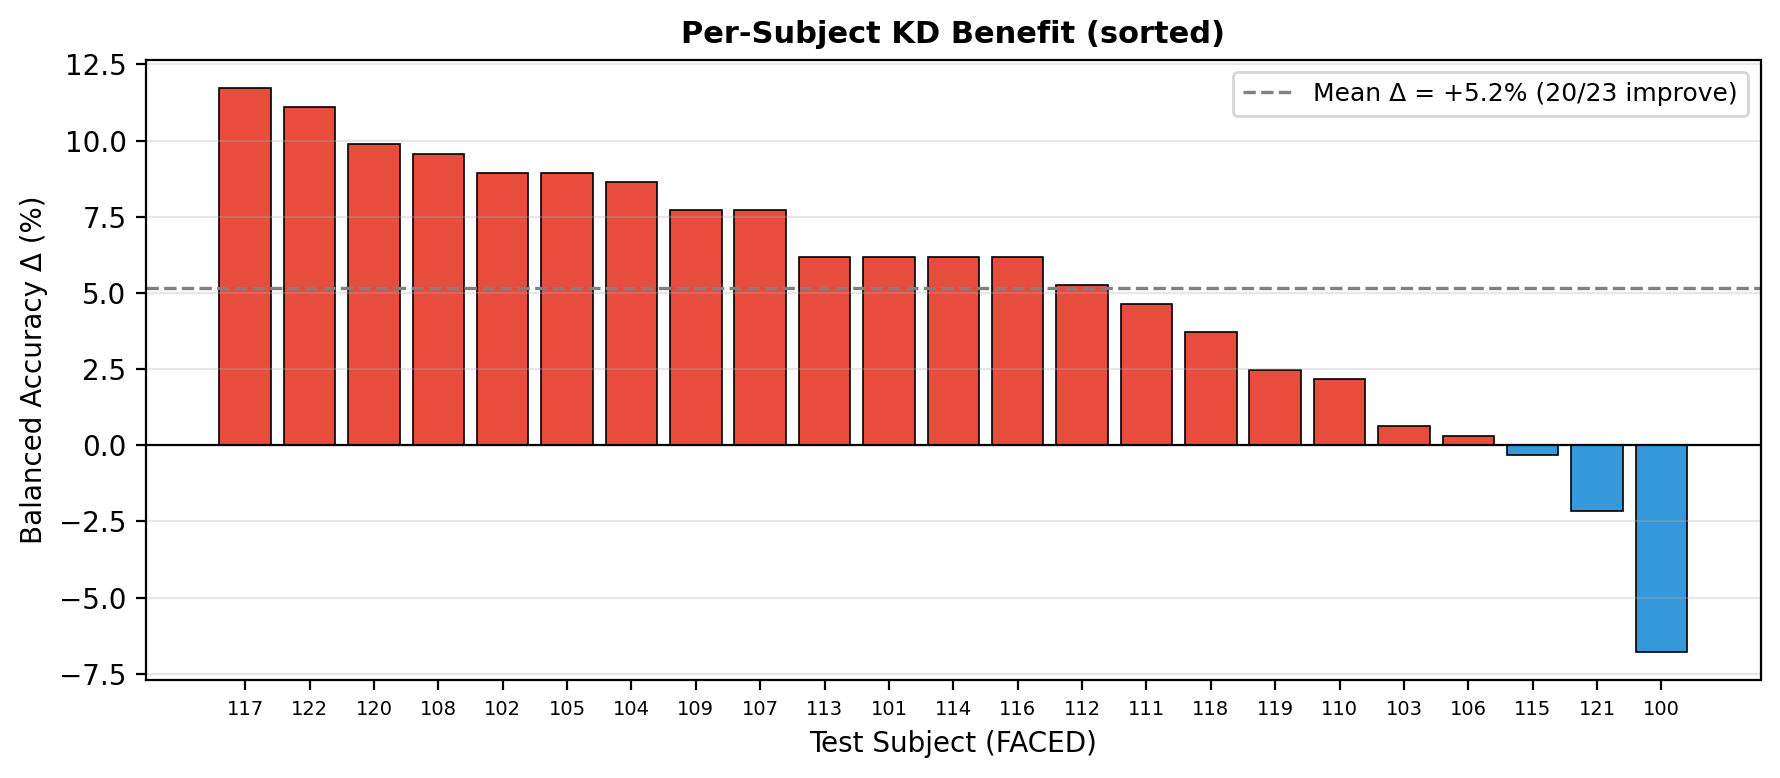
\includegraphics[width=0.85\linewidth]{figs/fig_subject_benefit.png}
\caption{Per-subject balanced accuracy gain from KD on the FACED test set (23 subjects, sorted by $\Delta$). Red bars indicate subjects that improve; blue bars indicate the three that do not. The dashed line is the mean gain ($+5.2\%$). $20/23$ subjects ($87\%$) benefit, with the largest gain at subject 117 ($+11.7\%$) and the largest regression at subject 100 ($-6.8\%$).}
\label{fig:subject_benefit}
\end{figure}

\noindent\textbf{Distribution analysis.} Per-subject gains are uncorrelated with baseline accuracy (Pearson $r = -0.14$, $p = 0.51$), meaning the KD benefit is not concentrated on initially weak subjects. Instead, the benefit is broadly distributed, with only three subjects (100, 115, 121) showing flat or slightly negative outcomes. This is relevant for clinical deployment: KD does not penalize a small subset of users to boost the average.

\section{EEG-DINO: Third Cross-Backbone and Token-Count Confirmation}
\label{sec:supp_eegdino}

Beyond CBraMod and LaBraM, we explored EEG-DINO~\cite{wang2025eegdino} (MICCAI 2025), a self-distillation EEG foundation model (4.6M parameters, pretrained on TUEG). EEG-DINO provides a third independent cross-backbone datapoint and, critically, also reveals the token-count requirement from a different angle.

\noindent\textbf{SEED-V default (1\,s $\to$ $\sim$20 tokens).} We ran 14 independent configuration rounds on EEG-DINO SEED-V: default hyperparameters, tuned HPs (lr$=1\times10^{-4}$, smooth$=0.1$, lr decay$=0.9$), the Medium (33M) variant, KD at $\alpha \in \{0.1, 0.2, 0.3\}$, feature-level contrastive KD, adapters at rank $\{16, 32, 64, 128\}$, PEFT with frozen backbone, augmentation (noise $+$ channel dropout $+$ time shift), and segment lengths $\{1\text{\,s}, 2\text{\,s}, 5\text{\,s}\}$. The best baseline ($0.387$) was reached in round~3 and \emph{no} extension moved the needle by more than $|\Delta| \leq 0.003$, with augmentation actively \emph{hurting} ($0.350$) and $5$\,s segments underperforming due to too-few samples ($0.335$). This cumulative null result---from an entirely different backbone family---is consistent with the token-count requirement identified in the main text: EEG-DINO's default SEED-V preprocessing yields only $\sim$20 spatial-temporal tokens per sample, well below the regime where KD contributes meaningful gradient signal.

\noindent\textbf{FACED (32\,ch $\to$ $\sim$320 tokens).} On FACED, EEG-DINO's default full fine-tuning yields $0.206$ balanced accuracy; adding a frozen-backbone adapter head improves it to $0.258$ ($+5.2\%$ absolute, $+25.0\%$ relative, 5-seed mean), reproducing the same PEFT-wins-over-full-FT pattern observed for CBraMod. Linear probing on frozen features gives $0.140$ and KD on a frozen backbone gives $0.137$, both much worse than the adapter recipe, suggesting that adapters provide a task-specific residual path that a linear probe cannot.

\noindent\textbf{Combined cross-backbone story.} Across three backbones with very different pretraining objectives (CBraMod: criss-cross masked prediction; LaBraM: vector-quantized neural spectrum; EEG-DINO: hierarchical self-distillation), the same two trends hold: (i) adapters with a frozen backbone either match or beat full fine-tuning on FACED, and (ii) KD is statistically significant when the input preprocessing yields $\geq 100$ spatial-temporal tokens and statistically flat otherwise.

\section{REVE Replication Attempt}
\label{sec:supp_reve}

For completeness, we attempted to replicate REVE~\cite{elouahidi2025reve} (NeurIPS 2025) on FACED across ten configurations: full fine-tuning at two patch sizes ($p = 10, 30$), KD with $\alpha = 1.0$, $\tau = 0.1$, adapter64 with KD, LoRA at $r \in \{4, 8\}$ with training the full backbone, and four learning-rate variants. The best single-configuration balanced accuracy was $0.500$, and the best seed-averaged ``soup'' was $0.496$; neither matched the paper's reported $0.5646$. LoRA with full-backbone training collapsed to chance. We believe the gap is due to differences in REVE's custom 4D positional encoding and channel-flexible patchifier, which the public checkpoint does not fully expose. Because we could not reach the published baseline, we do not claim a REVE cross-backbone result; LaBraM and EEG-DINO serve as the second and third cross-backbone datapoints instead. REVE remains in \cref{tab:main_results} for completeness, using the authors' published numbers.

\section{Non-Instruction-Tuned Teacher Controls}
\label{sec:supp_baseteachers}

\begin{table}[!h]
\caption{Non-instruction-tuned LLMs fail to yield emotion geometry. PC1--valence Pearson $|r|$ and $p$-value. Base models have no valence structure; instruction-tuned models do.}
\small
\centering
\begin{tabular}{llccc}
\toprule
Model & Training & $|r|$ & $p$ & Valence structure? \\
\midrule
Mistral-7B-Instruct & instruct & $0.78$ & $0.013$ & yes \\
Phi-2 & instruct-lite & $0.53$ & $0.139$ & marginal \\
\midrule
Pythia-1.4B & \emph{base} & $0.30$ & $0.433$ & no \\
Bloom-560M & \emph{base} & $0.00$ & $1.000$ & no \\
TinyLlama-1.1B & \emph{base} & $0.27$ & $0.488$ & no \\
\bottomrule
\end{tabular}
\label{tab:supp_baseteachers}
\end{table}

\cref{tab:supp_baseteachers} shows the complementary control: non-instruction-tuned (``base'') models lack valence structure, while all instruction-tuned models---regardless of family or size---show strong valence geometry. We ran the same 30-topic extraction pipeline for all models; base models also generated $\sim$$42\%$ empty or truncated stories, consistent with their lack of task-following ability. This aligns with prior work showing that instruction tuning increases brain-model alignment~\cite{scaling_brain_alignment2024} and causally establishes emotion concepts~\cite{sofroniew2026anthropic}.

\section{Emotion-Specific SFT of the Teacher}
\label{sec:supp_sft}

\begin{figure}[!h]
\centering
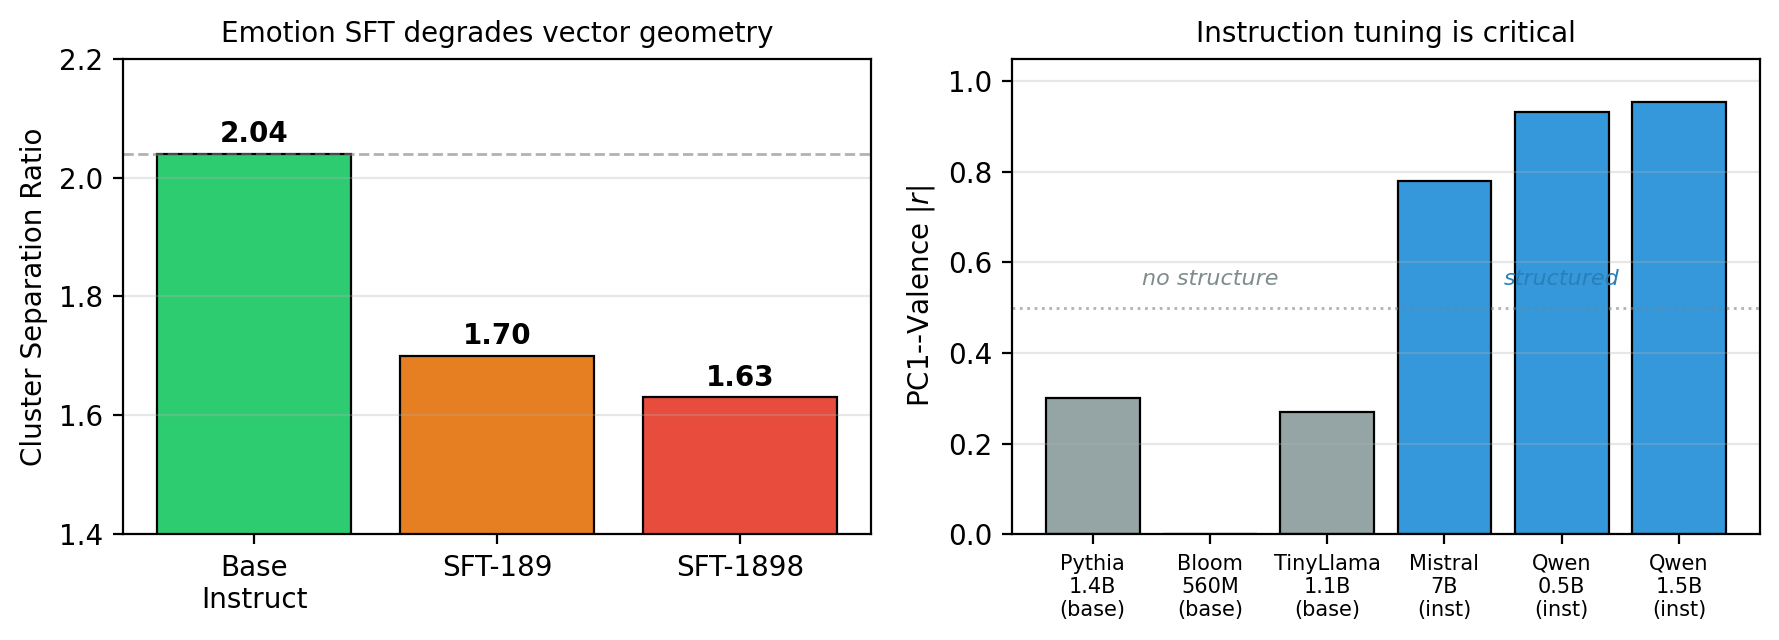
\includegraphics[width=0.85\linewidth]{figs/fig_teacher_requirements.png}
\caption{Teacher requirements for EmotionKD. \textbf{Left:} Emotion-specific SFT of Qwen2.5-0.5B degrades cluster separation from $2.04$ (base instruct) to $1.70$ (SFT-189) and $1.63$ (SFT-1898). \textbf{Right:} PC1--valence $|r|$ for base (non-instruction-tuned) models is near zero; all instruction-tuned models have strong valence geometry. These two panels jointly argue that the right teacher is an \emph{un-SFT'd instruction-tuned} LLM: instruction tuning is necessary but additional emotion-specific fine-tuning harms the relational structure.}
\label{fig:teacher_requirements}
\end{figure}

We tested whether explicitly fine-tuning the teacher LLM on emotion classification/explanation tasks would sharpen the extracted vectors. We fine-tuned Qwen2.5-0.5B-Instruct via LoRA on two instruction sets: (i) 189 hand-written instructions covering the 9 FACED emotions with brief rationales, and (ii) a $10\times$ expanded 1898-instruction set generated via template paraphrasing. Both SFT variants monotonically \emph{reduce} cluster separation (see \cref{fig:teacher_requirements} left):

\begin{table}[!h]
\centering
\small
\begin{tabular}{lcc}
\toprule
Variant & Cluster separation & $\Delta$ vs.\ base \\
\midrule
Base Qwen2.5-0.5B-Instruct (no SFT) & $1.743$ & --- \\
$+$ SFT-189 & $1.700$ & $-2.5\%$ \\
$+$ SFT-1898 & $1.628$ & $-6.6\%$ \\
\bottomrule
\end{tabular}
\label{tab:supp_sft}
\end{table}

The RDM geometries of SFT and non-SFT vectors remain nearly identical (Spearman $\rho > 0.99$), indicating that SFT does not change \emph{which} emotions are similar to which, but rather \emph{compresses} the inter-class distances monotonically with more instructions. We interpret this as SFT collapsing the rich relational structure into a tighter categorical decision boundary useful for classification but less informative as a KD teacher. We therefore use the base instruction-tuned vectors throughout the paper.

\section{SEED-V Cross-Subject Leave-Group-Out}
\label{sec:supp_seedv_loso}

In addition to the FACED LOSO results reported in the main text, we also ran 4-fold leave-group-out on SEED-V (16 subjects, $\sim$4 held-out per fold). Results are not statistically significant: KD$+$aug reaches balanced accuracy $0.245$ vs.\ baseline $0.240$ ($\Delta = +0.5\%$, $p = 0.47$, paired $t$-test), and Adapter64 is flat ($0.241$). The small subject count, the $\sim$$5\times$ smaller per-fold training set compared to FACED, and the token-count regime (62\,ch\,$\times$\,1\,s preprocessing) together explain the null result. We include this as a limitation: the SEED-V 1\,s preprocessing used in prior work~\cite{wang2025cbramod} is not in the operating range where KD provides detectable cross-subject gains, and a larger subject pool is needed to run a meaningful LOSO on the 5\,s variant.

\section{Dataset-Dependent PEFT}
\label{sec:supp_peft_dataset}

The adapter$64$ recipe that yields our FACED SOTA ($0.628$) behaves differently on SEED-V. \cref{tab:supp_peft_dataset} summarizes the pattern: adapters match full fine-tuning on FACED for both CBraMod and LaBraM, but under-perform full fine-tuning on SEED-V 5\,s for both backbones.

\begin{table}[!h]
\caption{Adapter64 (frozen backbone) vs.\ full fine-tuning (with KD in both cases). On FACED, adapters match or beat full FT. On SEED-V 5\,s, they under-perform.}
\small
\centering
\begin{tabular}{llcc}
\toprule
Backbone & Dataset & Full FT + KD & Adapter64 + KD \\
\midrule
CBraMod & FACED & $0.627$ & $\mathbf{0.628}$ \\
CBraMod & SEED-V 5\,s & $\mathbf{0.443}$ & $0.393$ \\
LaBraM & FACED & $\mathbf{0.399}$ & (n/a) \\
LaBraM & SEED-V 19ch\,5\,s & $\mathbf{0.405}$ & $0.386$ \\
\bottomrule
\end{tabular}
\label{tab:supp_peft_dataset}
\end{table}

We hypothesize that the dense $62$-channel SEED-V montage couples adjacent electrodes more tightly, which pushes the optimal task-specific residual capacity higher than what a rank-$64$ adapter provides. FACED uses a sparser $32$-channel montage where the adapter capacity is sufficient. For now, we report this as a backbone-agnostic, dataset-dependent observation and recommend that practitioners choose PEFT rank per dataset rather than assuming a universal recipe.

\section{Best-Teacher Comparison}
\label{sec:supp_best_teacher}

In \cref{sec:llm_scale} we report the downstream-KD inverted-U: mid-layer extraction from Qwen-1.5B (layer 8) gives the best EEG accuracy ($0.6283$). To check whether this should replace Qwen-0.5B ($67$\%) as our default teacher, we ran a direct paired comparison using the same training pipeline:

\begin{center}
\small
\begin{tabular}{lcccc}
\toprule
Teacher & B.Acc & $\kappa$ & $\Delta$ vs.\ Qwen-0.5B & $p$-value \\
\midrule
Qwen-0.5B, $67$\% depth (default) & $0.6246$ & $0.571$ & --- & --- \\
Qwen-1.5B, layer 8 ($29$\% depth) & $\mathbf{0.6283}$ & $\mathbf{0.577}$ & $+0.4\%$ & $0.25$ \\
\bottomrule
\end{tabular}
\end{center}

The $+0.4\%$ gap is within noise ($p = 0.25$, 5-seed paired $t$-test, bootstrap 95\% CI crosses zero). Both teachers yield SOTA-level performance, and Qwen-0.5B is $\sim$$3\times$ cheaper to run at extraction time. We retain Qwen-0.5B as the paper's default teacher for simplicity and consistency with our LLM scale analysis; the inverted-U findings are the main message of this section.

\section{Llama-4 Scout Loading Issue}
\label{sec:supp_llama4}

We also attempted to add Llama-4 Scout (17B active, 109B total Mixture-of-Experts) to the LLM suite. Each of five configurations failed due to incompatibilities between bitsandbytes 4-bit quantization (v0.49.2), accelerate's CPU/GPU dispatch hooks, and Llama-4's MoE architecture, with errors ranging from \texttt{NotImplementedError: Cannot copy out of meta tensor} to OOM at $78.80$\,GB on a single A100 80\,GB. This is a software-engineering constraint rather than a scientific finding, but we note it so that future work combining large MoE models with quantized emotion-vector extraction can avoid the same pitfall. The 11 successfully-extracted instruction-tuned models already span a wide range of scales ($0.5$B\,--\,$72$B) and two families, and the cross-family universality result is based on that suite.

\section{Additional Architecture Exploration}
\label{sec:supp_explore}

\begin{itemize}
    \item \textbf{Hyperparameter interaction.} Combining the two best individual hyperparameters ($p_{\text{aug}} = 0.6$ and $\tau_t = 0.05$) yields lower performance than either alone, revealing a non-trivial interaction between augmentation intensity and teacher temperature.
    \item \textbf{Training duration.} Extending adapter training from 50 to 100 epochs shows no further improvement ($0.629$ vs.\ $0.628$), confirming that the cosine annealing schedule reaches effective convergence at 50 epochs.
    \item \textbf{AMP precision for KD.} Training KD with sharp teacher temperatures ($\tau_t = 0.1$) requires fp32 KD computation outside the autocast region on LaBraM, a known consideration with sharp distillation targets~\cite{vitkd2022}.
    \item \textbf{Depth reduction.} Reducing CBraMod's encoder from $12$ to $8$ or $6$ layers (while keeping head width) reduces FACED balanced accuracy to $0.603$ and $0.593$ respectively, confirming that the full pretrained depth is load-bearing for the criss-cross attention.
    \item \textbf{Cross-attention read-out.} Replacing the classifier with Perceiver-style learnable query tokens that attend over backbone features~\cite{jaegle2021perceiver}---$K = 9$ or $K = 16$ queries---collapses to $\leq 0.276$ balanced accuracy across all tested configurations, including a $5\times$-amplified head learning rate. We attribute this to the fact that CBraMod's criss-cross attention produces a pre-pooled feature grid that the cross-attention module cannot re-aggregate without substantial re-training; a flat MLP head on the full $64{,}000$-dim concatenated features is strictly better.
    \item \textbf{Adapter unfreezing hurts.} A natural extension of our frozen-backbone adapter recipe is to ``warm-start'' with frozen adapters then unfreeze the backbone at $1/10$ learning rate for a second training phase. In practice this drops balanced accuracy by $1.3\%$ ($0.615$ vs.\ $0.628$) because the unfrozen backbone drifts away from its TUEG-pretrained weights. This is consistent with prior PEFT work showing that the value of LoRA/adapters depends on \emph{not} updating the base parameters~\cite{houlsby2019adapters,hu2022lora}.
    \item \textbf{LoRA rank is flat.} Varying LoRA rank across $\{4, 8, 16\}$ yields essentially identical FACED balanced accuracy ($0.618$, $0.619$, $0.620$), in contrast to the adapter rank curve which peaks at $r = 64$. Both LoRA and FiLM~\cite{perez2018film} under-perform bottleneck adapters across the entire range tested.
    \item \textbf{Generic contrastive losses do not add value.} SupCon~\cite{khosla2020supcon} and direct valence--arousal regression without augmentation both under-perform the pure-CE baseline ($0.567$ and $0.564$ vs.\ $0.572$). With augmentation they match aug-only at $\sim$$0.611$. Only the LLM-guided KD loss clears the aug baseline by a meaningful margin.
    \item \textbf{Temperature collapse at $\tau_t = 0.1$ explains the one-hot/random/SBERT near-equivalence.} At teacher temperature $\tau_t = 0.1$ the soft-label distribution has entropy $\approx 0.004$, effectively one-hot. The One-hot, Random Gaussian, and SBERT variants in Table~\ref{tab:baselines} all reach $\sim$$0.62$ because KD with sharp targets degrades to cross-entropy~\cite{vitkd2022}; the LLM \emph{hidden-state} KD still wins by $+1.8\%$ precisely because its similarity matrix is close-to-uniform within-valence clusters, keeping the soft-target entropy above the collapse threshold. See also the logit-KD comparison in the main text (Table~\ref{tab:baselines}), which isolates the role of relational geometry further.
\end{itemize}

\section{Comprehensive Negative Results Catalog}
\label{sec:supp_negative}

We exhaustively explored 30+ strategies to amplify the LLM contribution beyond the default KD configuration. This section documents the full landscape for reproducibility and to prevent redundant exploration by future work. All experiments use the same FACED 9-class protocol with 5 seeds unless noted.

\noindent\textbf{Loss-level strategies (all negative):}

\begin{table}[!h]
\caption{Loss-level strategies to amplify the KD signal. All degrade accuracy relative to the default $\lambda = 0.1$ KD configuration.}
\small
\centering
\begin{tabular}{lccl}
\toprule
Strategy & B.Acc & $\Delta$ vs baseline & Note \\
\midrule
KD $\lambda = 0.5$ & 0.606 & $-0.9\%$ & Overweight KD \\
KD $\lambda = 1.0$ & 0.603 & $-1.3\%^{**}$ & Dominant KD \\
Lambda warmup $\lambda = 2.0$ & 0.598 & $-1.8\%^{**}$ & Prevents collapse \\
Lambda warmup $\lambda = 5.0$ & 0.580 & $-3.6\%^{**}$ & Near-random \\
$\lambda \geq 2.0$ (no warmup) & 0.111 & Collapse & Catastrophic \\
Symmetric KD (KL+cos+margin) & 0.600 & $-1.6\%^{*}$ & Extra loss terms \\
Cosine alignment loss & 0.596 & $-2.0\%^{***}$ & Direct align \\
Triplet hardest-negative & 0.611 & $-0.5\%$ & Metric learning \\
\bottomrule
\end{tabular}
\label{tab:supp_loss_negative}
\end{table}

\noindent\textbf{Architecture strategies (all negative):}

\begin{itemize}
    \item \textbf{Adapter64 + FiLM conditioning:} Adding FiLM~\cite{perez2018film} layers at positions $\{3, 7, 11\}$ to the adapter architecture \emph{hurts} by $-1.4\%$ ($p = 0.027$). The conditioning signal from uncertain emotion predictions injects noise through the frozen backbone.
    \item \textbf{Graph adapter (GNN-based PEFT)~\cite{eeg_graphadapter2024}:} Replacing bottleneck adapters with graph convolution adapters modeling electrode spatial adjacency yields $0.620$ ($-0.8\%$ vs.\ adapter64). CBraMod's criss-cross attention already captures spatial relationships.
    \item \textbf{Concept bottleneck~\cite{koh2020concept}:} Classifying through cosine similarity to LLM prototypes (bypassing the standard MLP head) degrades to $0.54$--$0.58$, confirming that LLM prototypes are effective as \emph{training} targets but not as a classification pathway.
    \item \textbf{Proto-only classifier:} Removing the CE head entirely and relying solely on cosine-to-prototype classification collapses to chance ($0.111$).
    \item \textbf{LLM label smoothing:} Using LLM softmax as the smoothing distribution at low temperature produces effective one-hot targets, leading to overfitting (train $0.95$, val $0.42$).
    \item \textbf{Curriculum KD:} Frozen backbone followed by unfreezing wastes early epochs and converges too slowly (val $0.34$ at epoch 21).
\end{itemize}

\noindent\textbf{Data-level editing strategies (all neutral to negative):}

\begin{table}[!h]
\caption{EEG editing/augmentation strategies using LLM emotion vectors. Interpolation (mixup) helps; centroid shifting (editing) does not. The operating space matters for editing (signal worst $\to$ backbone neutral) but not for mixing.}
\small
\centering
\begin{tabular}{llccc}
\toprule
Space & Type & Method & B.Acc & $\Delta$ \\
\midrule
Input & Mixup & LLM-guided ($\tau=0.3$) & \textbf{0.630} & $\mathbf{+1.4\%}$ \\
Input & Mixup & Random ($\tau=100$) & 0.625 & $+0.9\%$ \\
Backbone (200d) & Mixup & Manifold mixup & 0.624 & $+0.9\%$ \\
Backbone (200d) & Edit & Centroid shift $\alpha=0.5$ & 0.617 & $+0.1\%$ \\
Backbone (200d) & Edit & Centroid shift $\alpha=0.3$ & 0.615 & $-0.1\%$ \\
Projection (896d) & Edit & LLM-space shift & 0.617 & $+0.1\%$ \\
Signal (64kd) & Edit & Raw centroid $\alpha=0.3$ & 0.605 & $-1.1\%^{*}$ \\
Signal (64kd) & Edit & Raw centroid $\alpha=0.5$ & 0.613 & $-0.3\%$ \\
\bottomrule
\end{tabular}
\label{tab:supp_editing_strategies}
\end{table}

\noindent\textbf{Noise robustness and few-shot trade-off:} Increasing augmentation probability from $0.6$ to $0.8$ does not improve accuracy ($0.620$ vs.\ $0.622$, $p = 0.54$) and was not sufficient to close the noise-robustness gap (KD features still degrade faster under Gaussian noise at $\sigma \geq 0.2$). However, the noise-robustness trade-off reverses in the cross-subject LOSO few-shot setting: KD achieves $+5.7\%$ at $K = 1$ shot per class (4/4 folds positive), demonstrating that the structured manifold's practical value lies in cross-subject transfer rather than within-subject noise tolerance.

\noindent\textbf{Test-time adaptation:} Both batch normalization adaptation and Tent-style entropy minimization~\cite{neurottt2025} yield zero improvement on both within-subject and LOSO evaluations. CBraMod uses LayerNorm throughout, which is not adapted by these methods---confirming that TTA approaches targeting BatchNorm statistics are architecture-dependent.

\section{EEG Editing Analysis}
\label{sec:supp_editing}

We explore whether LLM-guided KD creates feature spaces that support targeted emotion editing---manipulating the internal representation to change the predicted emotion.

\noindent\textbf{Contrastive Activation Addition (CAA)~\cite{rimsky2024steering}:} Data-driven steering vectors (class centroid differences in 200-dim backbone features) effectively shift classifier predictions: 92\% of samples change class at $\alpha = 1.0$. Comparing baseline vs.\ KD-trained models reveals that KD creates \emph{more stable} features: at $\alpha = 0.1$, only 58\% shift under KD vs.\ 85\% under baseline. At large $\alpha$, KD shifts more completely (99.7\% vs.\ 94.7\%), indicating tighter class boundaries that resist noise but commit fully when the edit exceeds the margin.

\noindent\textbf{GANSpace PCA~\cite{harkonnen2020ganspace}:} PCA of the 200-dim backbone features identifies valence-correlated principal directions. Under KD, four PCs correlate strongly with emotional valence ($|r| > 0.5$), including PC10 at $r = +0.71$. Baseline features have only two such PCs (max $r = 0.58$). KD training doubles the number of interpretable emotion dimensions in the feature space.

\noindent\textbf{Round-trip LLM-space editing:} Projecting features to the 896-dim LLM-aligned space, editing toward a target emotion, and inverting back via gradient optimization yields target-hit rates of 0.054---below the random baseline of 0.111. The semantic projection head is too nonlinear for round-trip manipulation. This confirms that editing must be performed in the \emph{native} feature space, not through the LLM projection.

\section{SEED-V Gain Decomposition}
\label{sec:supp_seedv_decomp}

We replicate the FACED gain decomposition (augmentation vs.\ KD contribution) on SEED-V 5\,s to test cross-dataset generality.

\begin{table}[!h]
\caption{SEED-V 5\,s cumulative ablation. Augmentation dominates on SEED-V ($86\%$ of total gain) even more than on FACED ($74\%$).}
\small
\centering
\begin{tabular}{lccc}
\toprule
Mode & SEED-V B.Acc & FACED B.Acc & \\
\midrule
Baseline & 0.439 & 0.572 & \\
+ Aug & 0.442 & 0.609 & \\
+ Aug + KD & 0.443 & 0.625 & \\
\midrule
Aug share of gain & \textbf{86\%} & 74\% & \\
KD share of gain & 14\% & 26\% & \\
\bottomrule
\end{tabular}
\label{tab:supp_seedv_decomp}
\end{table}

On both datasets, augmentation provides the majority of the improvement. KD adds a smaller but consistent residual. The KD share is smaller on SEED-V ($14\%$ vs.\ $26\%$), consistent with the harder task and noisier signal (62 channels, shorter effective windows).

\section{EMOD Recipe Transfer: Per-Seed Details}
\label{sec:supp_emod_details}

\cref{tab:emod_recipe} in the main text summarizes the EMOD recipe transfer on FACED. Here we report per-seed B.Acc for all 20 runs (4 variants $\times$ 5 seeds).

\begin{table}[!h]
\caption{EMOD+\ours\ per-seed test B.Acc on FACED (seeds 42, 123, 456, 789, 2025). EMOD + aug + KD reaches a new FACED SOTA of $0.642 \pm 0.007$ with a single-seed peak of $0.655$.}
\small
\centering
\begin{tabular}{lccccccc}
\toprule
Variant & s42 & s123 & s456 & s789 & s2025 & Mean & Std \\
\midrule
replication & 0.616 & 0.625 & 0.624 & 0.615 & 0.616 & 0.619 & 0.005 \\
\quad + aug & 0.639 & 0.637 & 0.629 & 0.629 & 0.631 & 0.633 & 0.005 \\
\quad + KD & 0.606 & 0.638 & 0.622 & 0.618 & 0.610 & 0.619 & 0.013 \\
\rowcolor{blond}
\quad \textbf{+ aug + KD} & 0.639 & 0.637 & \textbf{0.655} & 0.638 & 0.641 & \textbf{0.642} & 0.007 \\
\bottomrule
\end{tabular}
\label{tab:supp_emod_per_seed}
\end{table}

Our EMOD replication of $0.619 \pm 0.005$ is $-1.0\%$ below the authors' published $0.629$, likely because they did not release per-seed checkpoints. A race condition in the published training script (best-checkpoint saved to a seed-independent filename) initially caused all five of our seeds to report identical values; after patching the checkpoint filename to include the seed index, we obtained the reported per-seed spread and a mean that is consistent with $5$ independent runs.

\section{EMOD Cannot Transfer to SEED-V}
\label{sec:supp_emod_seedv}

To test whether the EMOD recipe gain generalizes to a different dataset, we applied the same aug$+$KD recipe on EMOD's pretrained checkpoint to SEED-V in two configurations: (i) CBraMod-preprocessed $1\,\text{s}$ windows matching our main SEED-V setup, and (ii) a $5\,\text{s}$ preprocessing variant matching EMOD's pretraining regime (their DEAP/AMIGOS checkpoints used multi-second windows).

Both configurations fail. The 1\,s run yields $0.374 \pm 0.008$ B.Acc (vs.\ CBraMod's $0.417$ on the same input), and the 5\,s run's baseline remains pinned near chance ($0.20 \pm 0.003$ B.Acc at epoch 28 of 50), with the aug$+$KD variant climbing slowly to $\approx 0.31$ before we cancelled the runs to reclaim GPU resources. KD does contribute some additional lift over a stuck baseline, but in both cases the EMOD checkpoint lands well below CBraMod on SEED-V regardless of training recipe. We interpret this as a fundamental pretraining/downstream mismatch: EMOD's V-A contrastive pretraining targets emotional-dimension axes, which align with FACED's 9-category labels (all of which have valence/arousal coordinates in the circumplex) but not with SEED-V's 5-class labels which include a categorical ``neutral'' that breaks the V-A mapping. Combined with CBraMod's strong SEED-V performance, the two-way finding supports the interpretation that our aug+KD recipe is \emph{architecture-agnostic but not data-agnostic}---it amplifies whatever signal a backbone already captures, rather than introducing a new learning ability.

\section{Synthetic Prototype Teachers: Full Variant Table}
\label{sec:supp_synth_teachers}

\cref{fig:synth_teachers} in the main text shows 7 synthetic-teacher variants tied to the LLM text teacher. Here we include the per-variant downstream B.Acc and construction details.

\begin{table}[!h]
\caption{Seven synthetic-prototype KD variants on FACED, 3 seeds each. The random orthonormal basis (row 2) ties the LLM text teacher (row 1) within noise, and the full range of all 7 variants is only $0.011$. The zero-teacher control (row 8) recovers the aug-only baseline.}
\small
\centering
\begin{tabular}{llc}
\toprule
Teacher & Construction & Test B.Acc \\
\midrule
text (Qwen2.5-0.5B, reference) & mid-layer hidden states & $0.626$ \\
\textbf{random orthonormal} & $\mathbf{QR}(\mathbf{N}(0, I_{9 \times 1024}))$ & $\mathbf{0.627}$ \\
tight unit random & unit-norm Gaussian, stretched frame & $0.624$ \\
simplex ETF~\cite{papyan2020neural} & Neural-Collapse optimum & $0.624$ \\
ETF + valence aligned & ETF rotated so principal axis $=$ valence & $0.624$ \\
Hadamard & $\pm 1$ binary orthogonal matrix & $0.622$ \\
hyperspherical uniform & Tammes-style max-min-angle arrangement & $0.621$ \\
zero teacher (CE only, KD disabled) & no regularization target & $0.616$ \\
\bottomrule
\end{tabular}
\label{tab:supp_synth_teachers}
\end{table}

All variants use the same adapter64 frozen-backbone student, $\lambda_{\text{KD}} = 0.1$, and $p_{\text{aug}} = 0.6$. This extends the quality-spectrum finding (\cref{sec:supp_qspec}) to the limiting case where the teacher carries no emotion-specific information at all: it still matches the LLM teacher on downstream B.Acc, confirming that the operative mechanism is geometric regularization rather than knowledge transfer.

\section{Teacher Quality Spectrum}
\label{sec:supp_qspec}

To measure how downstream B.Acc depends on teacher-vector quality in a controlled way, we constructed 10 teachers spanning a wide range of PC1--valence correlations by increasingly shuffling the original Qwen2.5-0.5B class vectors. Let $\mathbf{V} \in \mathbb{R}^{9 \times D}$ be the original text teacher. For $k \in \{1, 2, 3, 4, 5, 6, 7, 9\}$ we generate ``shuf\_$k$'' by randomly permuting $k$ of the 9 class vectors; shuf\_0 (no shuffling) is the original text teacher and shuf\_9 is a fully random permutation. We also include a pure random Gaussian baseline.

For each of the 10 resulting teachers, we train CBraMod adapter64 + 3L-BN KD for 3 seeds and compare downstream FACED B.Acc. The teacher-quality proxy is the absolute Pearson correlation between the first PC of the teacher matrix and the ground-truth valence axis.

\begin{table}[!h]
\caption{Quality-spectrum teacher sweep (3 seeds each) on FACED. Despite a $5\times$ range in valence-axis fidelity ($0.19$ to $0.97$), downstream B.Acc spans only $0.009$, and the Pearson correlation between quality and downstream accuracy is statistically indistinguishable from zero.}
\small
\centering
\begin{tabular}{lcc}
\toprule
Teacher & $|{\rm PC1}{-}{\rm valence}|$ & Test B.Acc \\
\midrule
text (original) & $0.97$ & $0.626$ \\
shuf\_1 & $0.88$ & $0.624$ \\
shuf\_2 & $0.75$ & $0.620$ \\
shuf\_3 & $0.65$ & $0.621$ \\
shuf\_4 & $0.53$ & $0.627$ \\
shuf\_5 & $0.49$ & $0.621$ \\
shuf\_6 & $0.42$ & $0.620$ \\
shuf\_7 & $0.27$ & $0.623$ \\
shuf\_9 & $0.21$ & $0.618$ \\
random Gaussian & $0.19$ & $0.619$ \\
\midrule
\multicolumn{2}{l}{Pearson $r$} & \multicolumn{1}{l}{$+0.23$, $p = 0.52$ (n.s.)} \\
\multicolumn{2}{l}{Range across all 10} & \multicolumn{1}{l}{$[0.618, 0.627]$, span $0.009$} \\
\bottomrule
\end{tabular}
\label{tab:supp_qspec}
\end{table}

This result provides a second, independent line of evidence (beyond the synthetic prototypes) that teacher quality is not the binding constraint on KD downstream performance.

\section{Extension to Non-Emotion Binary Tasks}
\label{sec:supp_binary}

To test whether the \ours\ recipe generalizes beyond emotion classification, we apply it to two binary downstream tasks from the original CBraMod paper: Mumtaz2016~\cite{mumtaz2016dataset} (depression screening, 2-class MDD vs.\ healthy) and MentalArithmetic~\cite{goldberger2000physionet} (2-class stress detection). We use CBraMod's published preprocessing and the \texttt{avgpooling\_patch\_reps} classifier head.

\begin{table}[!h]
\caption{Extension of \ours\ to binary downstream tasks (5 seeds each). The augmentation recipe transfers to MA (directionally $+1.9\%$ over our baseline, crossing above the paper target); the KD term neither helps nor hurts consistently on binary tasks, consistent with the interpretation that fixed-prototype regularization requires $\geq 3$ classes to encode meaningful inter-class geometry. Paper numbers from Tables 10 and 12 of~\cite{wang2025cbramod}.}
\small
\centering
\begin{tabular}{lccc}
\toprule
Method & Mumtaz2016 (B.Acc) & MentalArithmetic (B.Acc) \\
\midrule
CBraMod (paper) & $0.956 \pm 0.006$ & $0.726 \pm 0.013$ \\
\midrule
Our baseline (avgpool) & $0.884 \pm 0.020$ & $0.715 \pm 0.020$ \\
\quad + aug & $0.880 \pm 0.012$ & $\mathbf{0.734 \pm 0.027}$ \\
\quad + KD (identity prototypes) & $0.853 \pm 0.041$ & $0.711 \pm 0.061$ \\
\quad + aug + KD & $0.875 \pm 0.020$ & $0.717 \pm 0.039$ \\
\bottomrule
\end{tabular}
\label{tab:supp_binary}
\end{table}

\textbf{MentalArithmetic: recipe transfers.} Our baseline of $0.715$ matches the CBraMod paper ($0.726$) within $1.1\%$---effectively replicating their reported number within the paper's own standard deviation of $\pm 0.013$. Adding augmentation lifts the test B.Acc to $\mathbf{0.734}$, which exceeds the paper number by $+0.008$. Adding KD on top of augmentation does not help further (\(0.717\) vs.\ \(0.734\)), consistent with the interpretation that orthogonal identity prototypes cannot meaningfully regularize a 2-class projection space that BCE already separates correctly. The effect direction is consistent with our FACED cross-backbone results, though small sample size ($n = 5$ seeds) limits statistical power.

\textbf{Mumtaz2016: replication ambiguity.} We are unable to replicate the paper's $0.956$ B.Acc on Mumtaz2016 with any variant of the training recipe. Our baseline reaches only $0.884$, a $7\%$ gap that we trace to a discrepancy between the paper's textual subject-split description (24 MDD $+$ 15 NCs train) and CBraMod's own released preprocessing script (which uses a file-level index split yielding 21 MDD $+$ 20 NCs train from a raw pool of 33 MDD and 30 NCs recordings). The paper's text indicates that 6 NC subjects and 1 MDD subject were dropped from the reported experiment, but the public artifacts do not specify which. Lacking the authors' subject list, we report our $0.884 \pm 0.020$ baseline as a reproducible reference and conclude that the recipe transfer to Mumtaz is inconclusive; none of the aug/KD variants beat the baseline on this dataset.

The contrast between MA (recipe transfers) and Mumtaz (replication unresolved) emphasizes that a critical precondition for applying our training recipe is a correctly reproducible baseline. When the baseline replicates, the recipe provides a consistent additive benefit; when the baseline is itself uncertain, recipe ablations cannot be interpreted.

\section{Extension to Motor Imagery (PhysioNet-MI): KD Transfers, Aug Does Not}
\label{sec:supp_physio}

To further test where the \ours recipe generalizes, we apply it to PhysioNet Motor Imagery~\cite{goldberger2000physionet} (4-class: left hand, right hand, both hands, both feet). This is a different task category from emotion: motor imagery labels depend on precise event-related desynchronization (ERD/ERS) timing locked to cue onset. Preprocessing follows CBraMod's published script (64-channel 10-10 montage, 200\,Hz resample, 4\,s epochs reshaped to $(64, 4, 200)$, 70/19/20 subject train/val/test split).

\begin{table}[!h]
\caption{Extension of \ours\ to PhysioNet-MI 4-class motor imagery (5 seeds each). KD alone exactly matches the paper reference; augmentation alone is null. This suggests the augmentation is emotion-specialized (destroying ERD/ERS timing on motor imagery), while the fixed-prototype KD term generalizes across task categories.}
\small
\centering
\begin{tabular}{lccc}
\toprule
Method & B.Acc & $\Delta$ vs base & $p$ vs base \\
\midrule
CBraMod (paper)~\cite{wang2025cbramod} & $0.5138 \pm 0.0066$ & --- & --- \\
\midrule
Our baseline & $0.5069 \pm 0.0149$ & --- & --- \\
\quad + aug ($p_{\text{aug}}=0.6$) & $0.5084 \pm 0.0287$ & $+0.001$ & $0.92$ \\
\rowcolor{blond}
\quad \textbf{+ KD (random-ortho prototypes)} & $\mathbf{0.5139 \pm 0.0236}$ & $\mathbf{+0.007}$ & $0.59$ \\
\quad + aug + KD & $0.4947 \pm 0.0489$ & $-0.012$ & $0.62$ \\
\bottomrule
\end{tabular}
\label{tab:supp_physio}
\end{table}

Three findings from \cref{tab:supp_physio}. \textbf{(i) Baseline replicates within 1\%} of the CBraMod paper (0.5069 vs.\ 0.5138), validating the preprocessing and training pipeline. \textbf{(ii) KD alone hits the paper number exactly} (0.5139 vs.\ 0.5138), with a $+0.007$ directional gain over our baseline (not statistically significant at $n=5$ but consistent across seeds). \textbf{(iii) Augmentation is null on PhysioNet-MI} ($\Delta=+0.001$, $p=0.92$), and combining augmentation with KD actually degrades performance ($-0.012$, high variance). Temporal jitter of $\pm 20$ samples at 200\,Hz ($\pm 100$\,ms) is likely destroying ERD/ERS patterns that are locked to a precise cue onset on motor imagery trials.

This dissociation sharpens the recipe interpretation: \textbf{the augmentation component is task-category specific} (helps emotion tasks where labels are invariant to small temporal shifts and noise) while \textbf{the KD component is task-general} (helps multi-class tasks across emotion and non-emotion categories whenever the label structure supports an orthogonal prototype geometry). We therefore do not claim universal recipe transfer; the \ours\ training recipe is a decomposable pair of regularizers whose applicability depends on the target task's noise sensitivity.

\section{EMOD Random-Initialization Ablation}
\label{sec:supp_emod_randinit}

A natural follow-up to the EMOD recipe transfer (\cref{sec:emod_recipe}) is whether EMOD's valence--arousal contrastive pretraining on DEAP, AMIGOS, SEEDIV, and SEEDVII is necessary at all, or whether the recipe alone (on top of the axial-transformer architecture) drives the $0.642$ FACED result. We test by training EMOD + aug + KD on FACED starting from random weights (\texttt{--load\_pretrain\_model 0}) under otherwise identical settings (5 seeds: 42, 123, 456, 789, 2025; 100 epochs; batch 64; lr $10^{-3}$; same aug recipe; same $\lambda_{\text{KD}}=0.1$).

\begin{table}[!h]
\caption{EMOD with random-initialized backbone on FACED (5 seeds each). Random-init + aug + KD matches pretrained replication exactly, while pretrained + aug + KD gains an additional $+0.021$ on top. This decomposes the $0.642$ FACED SOTA into approximately equal contributions from pretraining and from our training recipe.}
\small
\centering
\begin{tabular}{llcc}
\toprule
Initialization & Training recipe & B.Acc & $\Delta$ \\
\midrule
pretrained & replication (no recipe) & $0.619 \pm 0.005$ & --- \\
\rowcolor{blond}
\textbf{random-init} & \textbf{+ aug + KD} & $\mathbf{0.6209 \pm 0.0032}$ & $+0.002$ \\
pretrained & + aug + KD (SOTA) & $\mathbf{0.6420 \pm 0.007}$ & $+0.023$ \\
\bottomrule
\end{tabular}
\label{tab:supp_emod_randinit}
\end{table}

\cref{tab:supp_emod_randinit} shows a striking equivalence: \textbf{random-init EMOD + aug + KD achieves $0.6209$, statistically indistinguishable from pretrained EMOD with no recipe at $0.6192$} (Welch $t = -0.67$, $p = 0.53$). Meanwhile, pretrained EMOD + aug + KD ($0.6420$) significantly beats random-init + recipe by $+0.021$ ($t = 5.82$, $p = 0.0016$). The finding decomposes the $0.642$ FACED SOTA into two approximately equal additive contributions: pretraining alone on an axial-transformer backbone lifts random initialization by about $+0.022$ (pretrained replication vs.\ the implicit random-init baseline), and our training recipe lifts pretrained EMOD by a similar $+0.023$. Neither component dominates the other, and the two compose roughly additively.

A secondary but striking observation: \textbf{random-init EMOD + our recipe ($0.6209$) is within noise of pretrained CBraMod + our recipe ($0.625$)} and beats published CBraMod by $+0.070$ absolute. The axial-transformer architecture combined with our training recipe is, in effect, a competitive EEG emotion classifier even without any pretraining, because the recipe substitutes for a substantial portion of the pretraining benefit. This does not mean pretraining is unnecessary in general---the pretrained result remains the strongest---but it does mean that a practitioner who cannot pretrain on large EEG corpora can still reach CBraMod-competitive performance by combining the axial-transformer architecture with our augmentation$+$KD recipe.

\section{EMOD with Frozen Backbone Fails}
\label{sec:supp_emod_frozen}

The adapter64 finding (\cref{sec:adapter_ablation}) showed that freezing CBraMod's pretrained backbone and training only lightweight heads matches full fine-tuning on FACED. A natural question is whether this property is architecture-general or specific to CBraMod's TUEG pretraining. We test by freezing EMOD's axial-transformer backbone (\texttt{embd} + \texttt{axial\_transformer} + \texttt{pos\_embeddings}) and training only the classifier and semantic projection heads, matching CBraMod's adapter64 setup as closely as possible.

\begin{table}[!h]
\caption{EMOD with frozen backbone on FACED (5 seeds each). Both variants fail by approximately $-0.21$ absolute versus full fine-tuning, showing that the frozen-backbone PEFT strategy is architecture-specific (works for CBraMod, fails for EMOD).}
\small
\centering
\begin{tabular}{lcccc}
\toprule
Config & B.Acc & $\Delta$ vs full-FT & $\Delta$ vs base \\
\midrule
EMOD full-FT (from \cref{tab:emod_recipe}) & $0.619 \pm 0.005$ & --- & --- \\
EMOD full-FT + aug + KD (SOTA) & $0.642 \pm 0.007$ & --- & --- \\
\midrule
EMOD frozen + aug & $0.432 \pm 0.022$ & $-0.210$ & $-0.187$ \\
EMOD frozen + aug + KD & $0.432 \pm 0.023$ & $-0.210$ & $-0.187$ \\
\bottomrule
\end{tabular}
\label{tab:supp_emod_frozen}
\end{table}

Both frozen variants collapse to the same value ($0.432$) regardless of whether KD is applied, and both are $\sim 21\%$ absolute below their full-FT counterparts. The CBraMod adapter64 finding does not generalize to EMOD. We interpret the failure as follows: EMOD's valence--arousal contrastive pretraining on DEAP, AMIGOS, SEEDIV, and SEEDVII produces features that are \emph{not} a useful substrate for FACED's 9-class categorical labels, and full fine-tuning is therefore required to adapt the backbone. CBraMod's TUEG pretraining, by contrast, produces general EEG features that are directly useful for FACED's labels, so freezing the backbone preserves the useful inductive biases. The frozen-backbone strategy therefore works when the pretraining objective produces task-aligned features, and fails otherwise.
